% Tipo de documento
\documentclass[12pt]{article}

% Configuracion de paquetes
\usepackage[T1]{fontenc}
\usepackage[utf8]{inputenc}
\usepackage[spanish, es-tabla]{babel}
\usepackage{amsmath}
\usepackage{amssymb, amsfonts, latexsym, cancel}
\usepackage{graphicx}
\usepackage{epstopdf}
\usepackage{float}
\usepackage{subfigure}
\usepackage{array, tabularx}
\usepackage{longtable}
\usepackage{bm}
\usepackage[lmargin=2cm, rmargin=2cm, top=2.5cm, bottom=2cm]{geometry}
\usepackage{fancyhdr}
\usepackage{enumerate}
\usepackage{listings}
\usepackage{multirow}
\usepackage{pgfplots}

% Configuracion de pagina
\parindent=0.5cm

% Configuracion de la graficadora
\pgfplotsset{width=14cm, compat=1.9}

% Modo de inicio y pie de pagina
\pagestyle{fancy}

\fancyhead{}
\fancyhead[C]{Tunel de viento}
\fancyhead[R]{
\includegraphics[scale=0.06]{src/institucion/Logo_uner-434x331.png}}
\renewcommand{\headrulewidth}{0.9pt}

\fancyfoot{}
\fancyfoot[R]{\thepage}
\fancyfoot[L]{Cristaldo M., Churruarin F., García F., Lovatto G. y Aguirre G.}
\renewcommand{\footrulewidth}{0.5pt}

% Inicio del documento
\begin{document}

% Inicio de la caratula
\begin{titlepage}
\begin{center}
% Nombre de la institucion
\vspace*{2\baselineskip}
\hrule height 3pt
\vspace*{0.5\baselineskip}
{\Huge \textbf{Presentación de proyecto N$^\circ$3}}
\vspace*{0.5\baselineskip}
\hrule
% Logo de la facultad
\vspace*{10\baselineskip}

\includegraphics[scale=0.35]{src/institucion/Logo_fcal-1174x247.png}
\vspace*{2\baselineskip}
% Nombre del trabajo y tipo
\textbf{\\TUNEL DE VIENTO\\}
\textbf{Laboratorio de mediciones}
% Nombre de los integrantes y fecha
\vfill
CRISTALDO M., CHURRUIARIN F., GARCÍA F., LOVATTO G. Y AGUIRRE G.\\
\today
\end{center}
\end{titlepage}

% Indice
\tableofcontents
\thispagestyle{empty}
\newpage

% Desarrollo del trabajo
\setcounter{page}{1}

% Introduccion
\section{Introducción}
Realizar un sistema de medición y control de temperatura en un tubo con mezcla de corrientes de aire fría y caliente con el fin de integrar los conocimientos adquiridos en la cátedra de Laboratorio de Mediciones Mecánicas, Eléctricas y Electrónicas, siendo los principales temas:

\begin{itemize}
	\item Medición de resistencias.
	\item Puentes de medición.
	\item Mediciones eléctricas de variables no eléctricas.
\end{itemize}

Además se pretende determinar la importancia de los sistemas de medida aplicados al control de procesos. 

% Alcance
\section{Actividad propuesta}
Esta práctica se realiza en el laboratorio de la facultad de la UNER, realizando la medición de temperatura, y caudal de un sistema de regulación proporcional.

% Teoria aplicada sugerida
\subsection{Teoria aplicada sugerida}
Apuntes de cátedra.

% Parámetros y rangos a determinar
\subsection{Parámetros y rangos a determinar}
\begin{itemize}
	\item Medición de temperatura.
	\item Medición de caudal.
\end{itemize}

% Equipos y aparatos
\subsection{Equipos y aparatos}
\begin{itemize}
	\item Instrumentos de medición disponibles en el laboratorio.
\end{itemize}

% Medidas de seguridad
\subsection{Medidas de seguridad}
\begin{itemize}
	\item Conectar los instrumentos a los alcances correspondientes según la medición a realizar.
	\item Conectar todo el circuito a una protección termomagnética y diferencial local en el banco de trabajo.
	\item Realizar la conexión y desconexión del circuito mediante interruptor.
	\item Evitar entrar en contacto con cualquier parte con tensión del circuito de medición y alimentación.
	\item Conectar la protección de tierra de seguridad donde corresponda.
	\item Cumplir las condiciones de seguridad previstas en el manual de seguridad del laboratorio para, instalaciones, equipos, instrumentos y personas. 
\end{itemize}

% Condiciones ambientales
\subsection{Condiciones ambientales}
Considerar las condiciones de temperatura ambiente para las mediciones realizadas.

% Procedimiento de la práctica
\subsection{Procedimiento de la práctica}
El grupo deberá construir el siguiente  sistema mezclador de corrientes de aire  y diseñar el sistema de medición y control de temperatura  de modo que el punto 3 se mantenga en un cierto rango de variación. El esquema es el siguiente:

\begin{figure}[H]
\centering
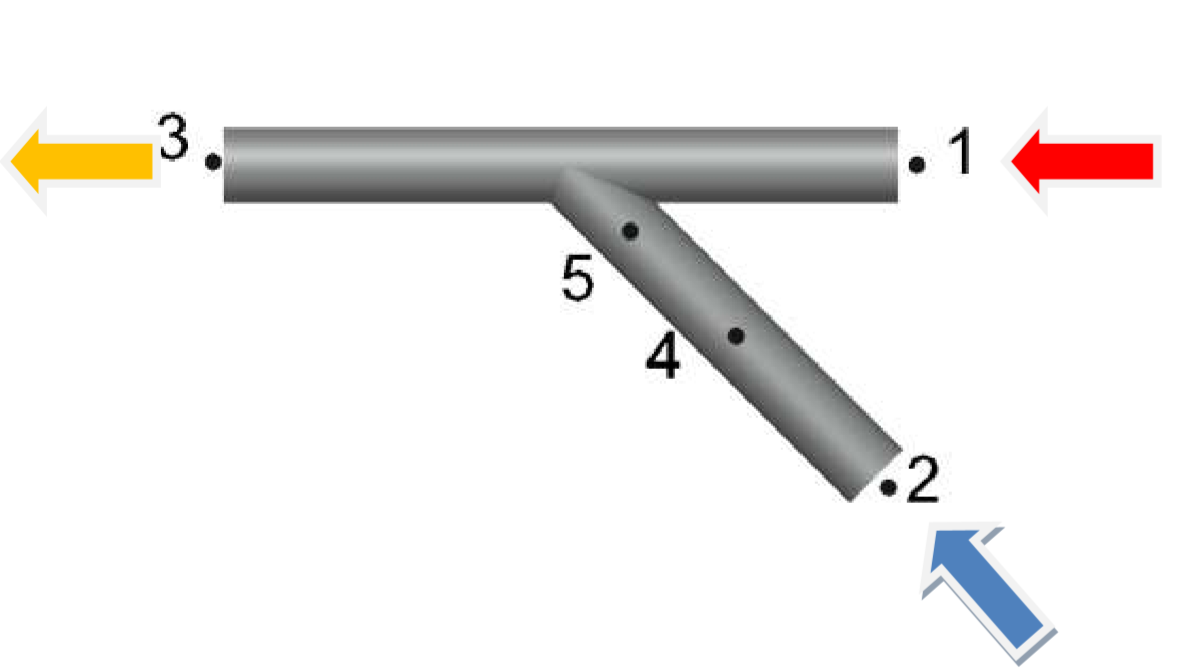
\includegraphics[scale=0.5]{../Imagenes/Tubos.png}
\caption{Esquema de conexión.}
\label{fgr:Tubos}
\end{figure}

\begin{enumerate}
	\item Ingreso de aire caliente a través de un ventilador a temperatura T1.
	\item Ingreso de aire frio a través de un ventilador a  temperatura T2.
	\item Salida de mezcla de aire  a  temperatura T3 definida por el usuario.
	\item Servomotor de apertura y cierre de aire a través de una clapeta.
	\item Medición de caudal a través de sistema de hilo caliente. 
\end{enumerate}

Se deberá construir el sistema de mezclador, para lo cual se colocaran dos ventiladores en el punto (1) y (2) de manera de obtener las corrientes de aire frio y caliente. Se deberá sensar la temperatura el punto (3), la cual deberá ser controlada dentro de un cierto rango establecido por el grupo, la cual se controla por la apertura y cierre de la clapeta (4).
Se deberá realizar el sensado de temperatura 1 y 2. Se deberá desarrollar un sistema de medición de caudal. 
La temperatura del punto (3) se conectara a través de conductores de longitud, no menor a 30 m. 
Todos los datos de medición se deberán visualizar a través de un display. 
Se deberán utilizar por lo menos dos tipos de sensores para la medición de temperatura (a elección). Se deberán construir el sistema de medición y diseñar el transductor correspondiente.

% Datos a ser registrados
\subsection{Datos a ser registrados}
Presentación de informe de laboratorio, con detalle de cálculos realizados, descripción de los sensores utilizados, puentes de medición, planos eléctricos, descripción de instrumentos utilizados, etc. 
Obtener conclusiones respecto a los resultados obtenidos.

% Incertidumbre
\subsection{Incertidumbre}
Se deberán analizar todas las fuentes posibles de error, realizando un estudio estadístico a la hora de presentar los resultados.

% Desarrollo
\section{Desarrollo}
Para lograr la construcción del artefacto, se tuvieron que llevar a cabo multiples tareas en paralelo asignadas al equipo.

% Esquema de funcionamiento
\subsection{Diagrama de flujo de funcionamiento}
El flujo de la información y la toma de deciciones del equipo está determinado como la ilustra la siguiente gráfica

\begin{figure}[H]
\centering
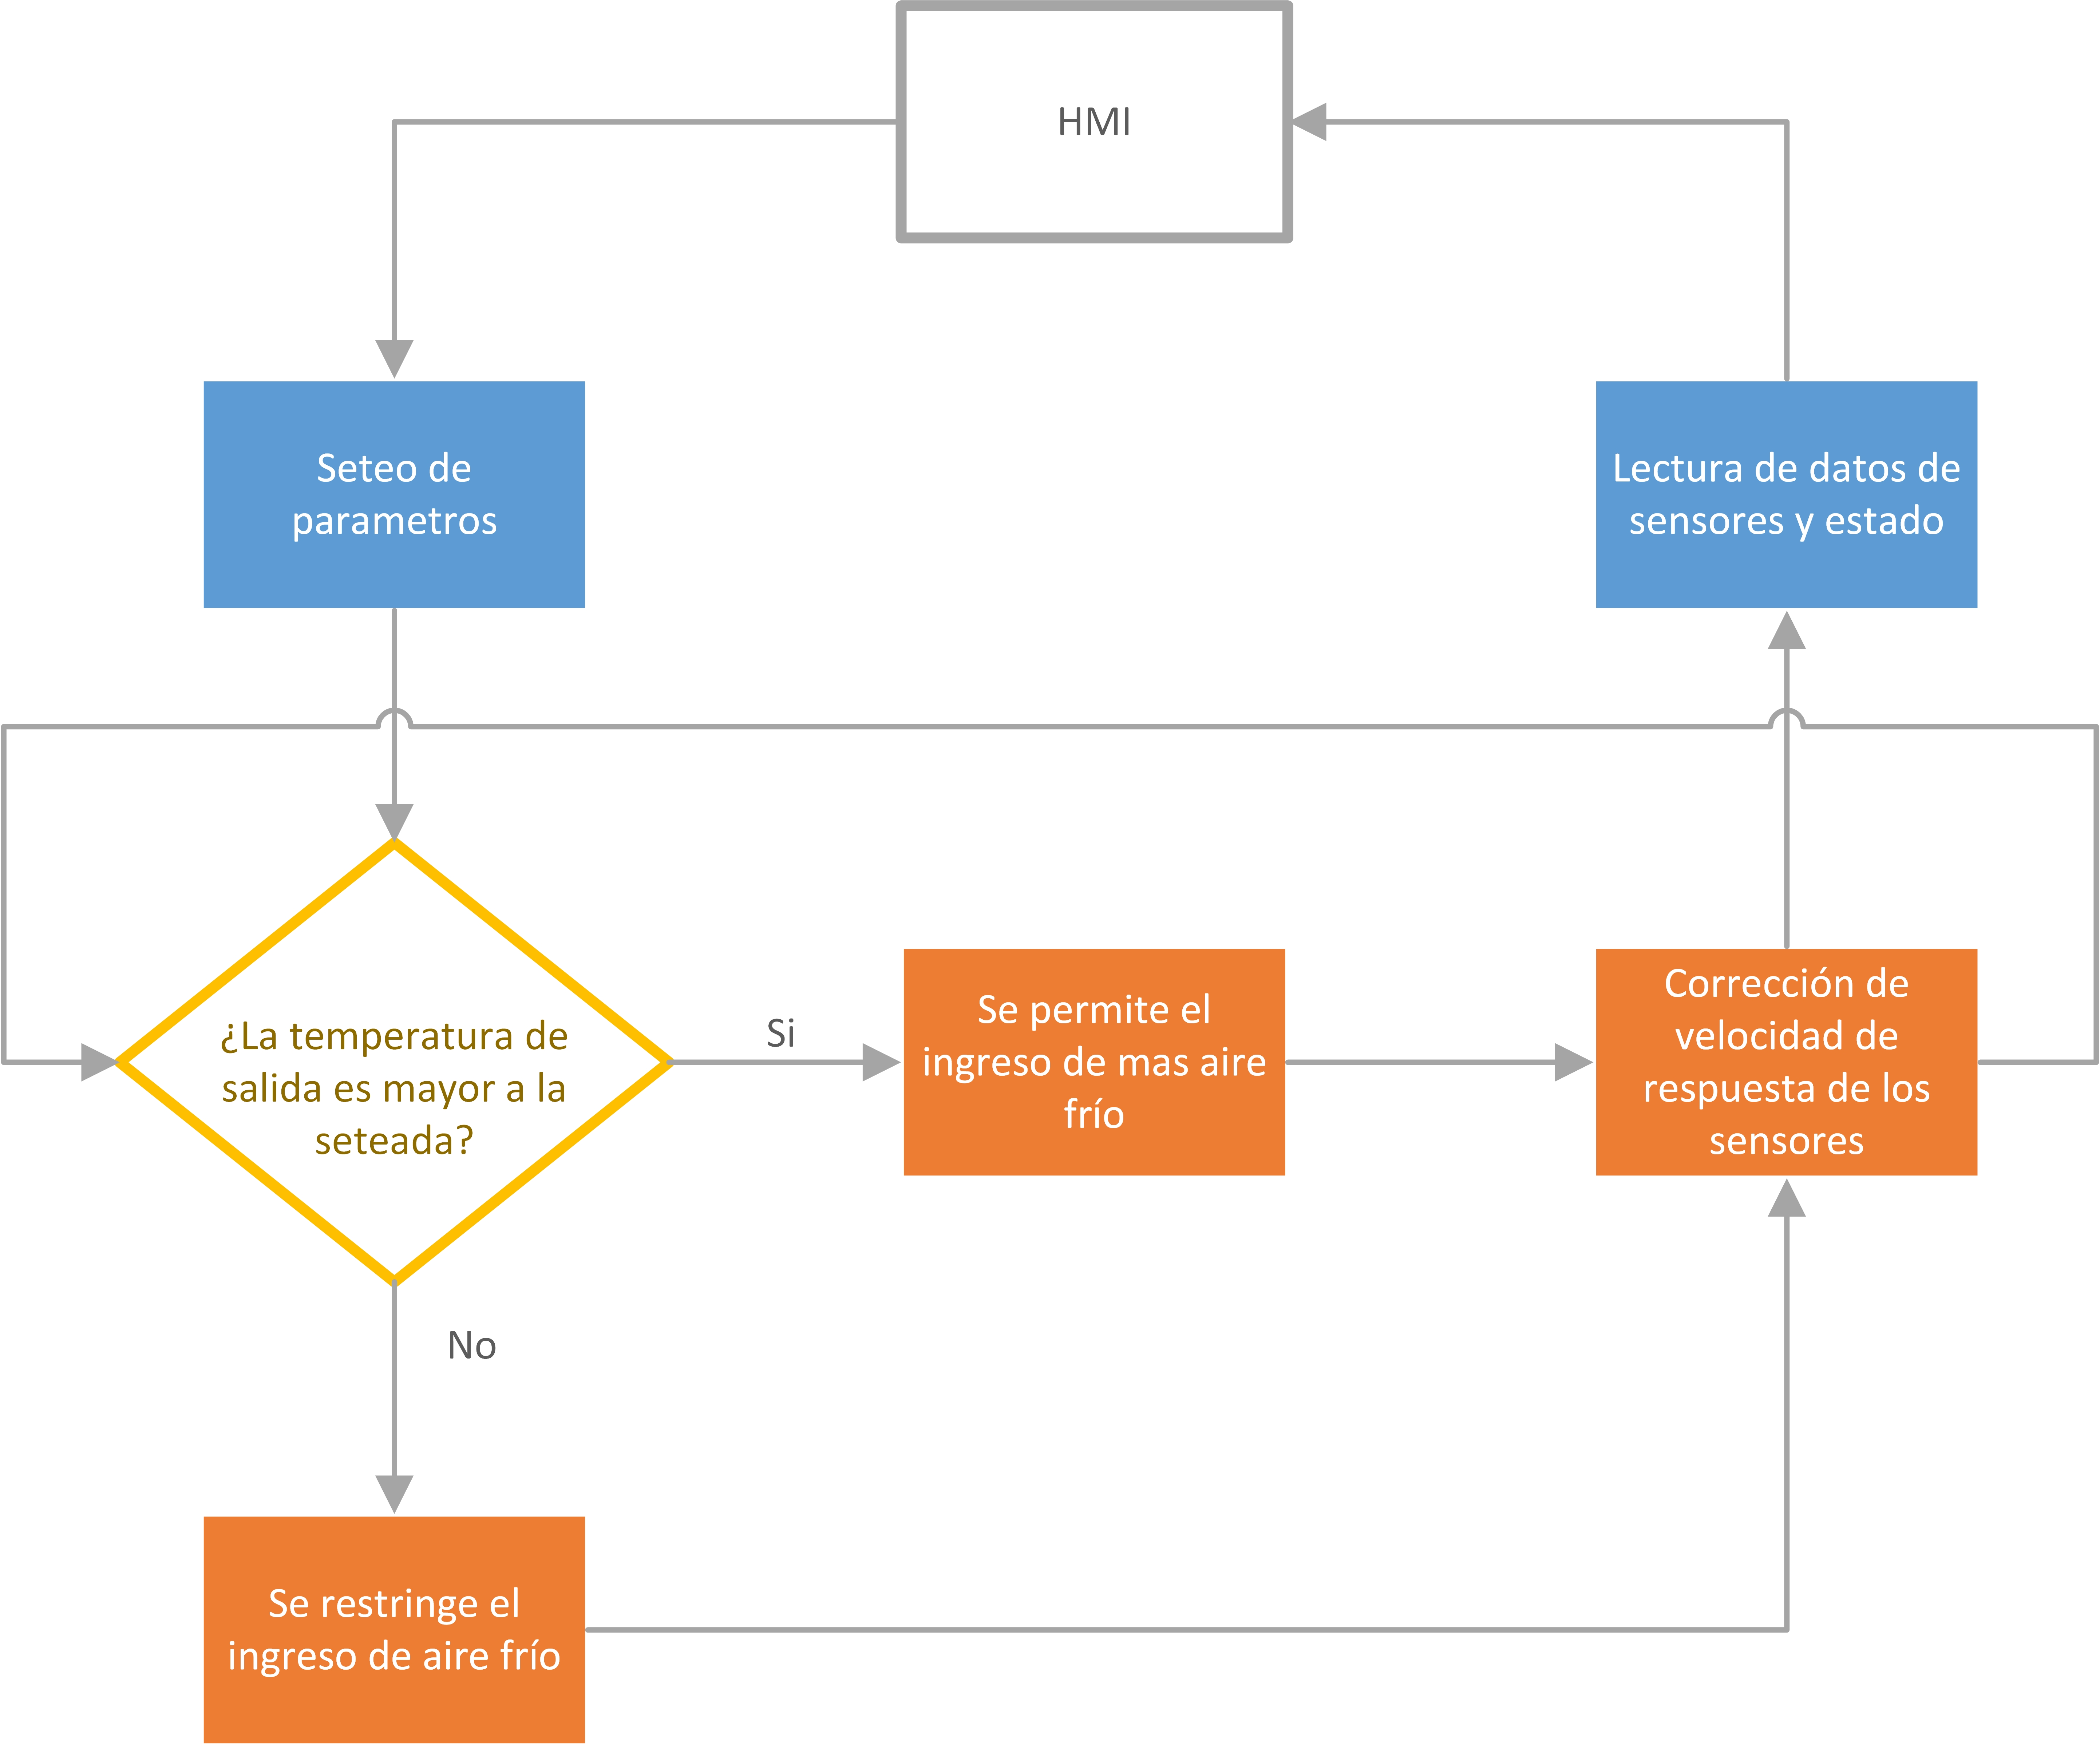
\includegraphics[scale=0.8]{src/imagenes/Flujo_principal.jpg}
\label{fgr:Flujo_principal}
\caption{Flujo principal del sistema.}
\end{figure}

El usuario interactua con el HMI y setea los parametros de funcionamiento, tales como la velocidad de respuesta, temperatura de salida y temperatura umbral. Con estos parametros el sistema realizara la mezcla optima entre la cantidad de aire frio y caliente. Los datos en tiempo real son mostrados en el esquema principal y las curvas de tendencia visualizadas en las gráficas.

% Linealizacion del sensor de temperatura NTC
\subsection{Sensor de temperatura (termistor)}

Existen dos tipos de termistor, las NTC y las PTC. Si solo mirásemos el nombre, la diferencia entre ambos es la primera letra N o P. Ambos nombres son siglas en inglés que significan:

\begin{itemize}
	\item \textbf{NTC:} Negative Temperature Coeficient
	\item \textbf{PTC:} Positive Temperature Coeficient
\end{itemize}

Otra diferencia es que la curva de calibración de la PTC es un poco menos amigable que la de la NTC. Esta curva no es más que la representación gráfica en la que enfrentamos la temperatura (en el eje Y) y la resistencia (en el eje X). Con ella apreciamos a simple vista la forma de comportarse del sensor. \\

En la mayoría de ocasiones en la que se debe usar un termistor, se opta por NTC, ya que aunque a priori puede parecer extraño tener una respuesta negativa, a la larga trae menos dolores de cabeza. \\

\subsubsection{Acondicionamiento y linealización del NTC}

Se trata de un sensor resistivo y por tanto, podemos usar varios circuitos distintos para realizar el acondicionamiento del sensor y obtener su lectura. \\

Como se trata de un sensor resistivo que no es de pequeña señal podemos usar las mismas técnicas que vimos para la LDR (fotoresistencia). \\

La primera posibilidad es usar una fuente de corriente. Esta técnica nos ayudará en la consistencia a lo largo del tiempo, y evitará aumentar la no linealidad. \\

La segunda posibilidad y la que vamos a usar en este caso es el circuito potenciométrico. Este circuito está formado por el sensor y una resistencia, colocadas en serie a modo de divisor de tensión. El circuito propuesto es el siguiente:

\begin{figure}[H]
\centering
\includegraphics[scale=0.6]{src/imagenes/Linealización_de_NTC.png}
\label{fgr:Flujo_principal}
\caption{Linealización del NTC por inclusión de resistencia en serie.}
\end{figure}

Este circuito es alimentado por una tensión, la cual provoca una tensión de salida en el punto medio del divisor de tensión (Tout). \\

\begin{equation*}
	R_{s} = \frac{\beta - 2 \cdot T_{o}}{\beta + 2 \cdot T_{o}} \cdot R_{o}
\end{equation*}

\begin{equation*}
	R_{25^{\circ}C} = 9.00K
\end{equation*}

\begin{equation*}
	R_{60^{\circ}C} = 2.32K
\end{equation*}

\begin{equation*}
	\beta = \frac{\ln{\left(\frac{9.00K}{2.32K}\right)}}{\frac{1}{300K} - \frac{1}{333K}} = 4145.73
\end{equation*}

\begin{equation*}
	R_{s} = \frac{4145.73 - 2 \cdot 333K}{4145.73 + 2 \cdot 333K} \cdot 2.32 \Omega \cdot 1000 = 1677.76 \Omega
\end{equation*}

El objetivo es calcular la temperatura, pero para llegar hasta ella debemos pasar por varias ecuaciones. Lo primero es conocer la tensión que hay en el punto medio del divisor de tensión y una vez conocida podremos calcular el valor de resistencia que presenta la NTC entre sus terminales. \\

Esto se puede hacer puesto que conocemos la tensión de alimentación y la resistencia fija. Todos estos parámetros se relacionan de la siguiente manera. \\

\begin{equation}
	\label{eqn:Resistencia_serie_NTC}
	V_{m} = V_{cc} \cdot \frac{R_{NTC}}{R_{aux} + R_{NTC}}
\end{equation}

Si despejamos $R_{NTC}$ de la ecuación \eqref{eqn:Resistencia_serie_NTC} nos queda  que la podemos calcular de la siguiente manera:

\begin{equation}
	\label{eqn:Resistencia_serie_NTC_despejada}
	R_{NTC} = \frac{R_{aux}}{\frac{V_{cc}}{V_{m}} - 1}
\end{equation}

Llegados a este punto, conocemos el valor de la resistencia que ofrece la NTC, sin embargo, el objetivo es conocer el valor de la temperatura a la que se ve sometida la NTC. 

\subsubsection{Ecuación de un termistor NTC}

Como casi todos los sensores que usamos en electrónica, los termistores NTC también disponen de un modelo matemático que nos ayuda a relacionar la resistencia entre sus terminales y la temperatura a la que se encuentra. \\

En el caso de las NTC, la relación entre la resistencia y la temperatura tiene una forma característica y difícil de olvidar, la cual se puede apreciar en su curva de calibración.

\begin{figure}[H]
\centering
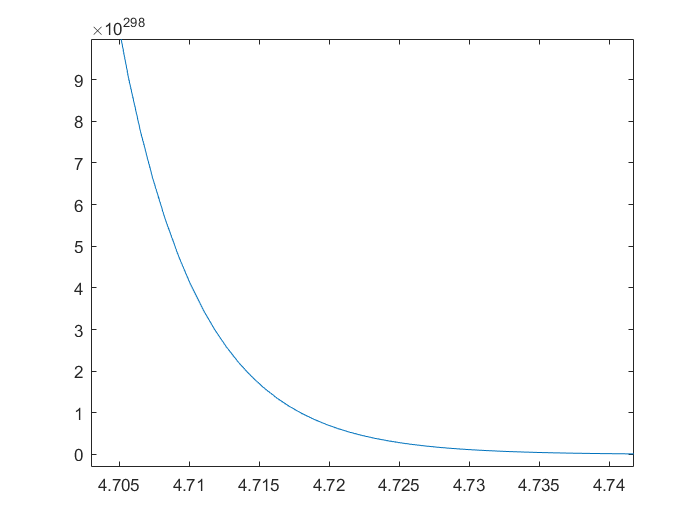
\includegraphics[scale=1]{src/imagenes/Curva_NTC.png}
\label{fgr:Curva_NTC}
\caption{Curva de resistencia de la NTC}
\end{figure}

Esta curva corresponde a una relación claramente exponencial y es por esto que la ecuación de las NTC es:

\begin{equation}
	\label{eqn:Curva_NTC}
	R_{NTC} = R_{0} \cdot e^{\beta \cdot (\frac{1}{T} - \frac{1}{T_{o}})}
\end{equation}

Donde:

\begin{itemize}
	\item $T_{o}$ es la temperatura de referencia, expresada en Kelvin.
	\item $R_{o}$ es la resistencia de referencia, es decir, la resistencia de la NTC cuando se encuentra a la temperatura de referencia.
	\item $\beta$ es la constante de la NTC
	\item $T$ es la temperatura que se está intentando medir, expresada en Kelvin.
\end{itemize}

\subsubsection{Calcular la temperatura}

Ahora, si aplicamos la ecuación \eqref{eqn:Curva_NTC}, podemos calcular cuanto debe ser la temperatura que está midiendo la NTC.

\begin{equation}
	\label{eqn:Temperatura_NTC}
	T = \left(\frac{\ln{(\frac{R_{NTC}}{R_{o}})}}{\beta} + \frac{1}{T_{o}} \right)^{-1}
\end{equation}

\subsubsection{Entrada al Arduino}

Se alimenta la entrada del sensor con $7V$ y a la salida del divisor obtenemos un rango de $5.11V$ a $80^{\circ}C$ y $1.4V$ a $25^{\circ}C$. Con este rango casi lineal de voltaje se puede extrapolar muy facilmente cualquier salida de tensión en una temperatura. \\

Las entradas analogicas del Arduino poseen como máximo un nivel de 5V, esto significa que la temperatura máxima medida puede ser de solo $75^{\circ}$.

\begin{figure}[H]
\centering
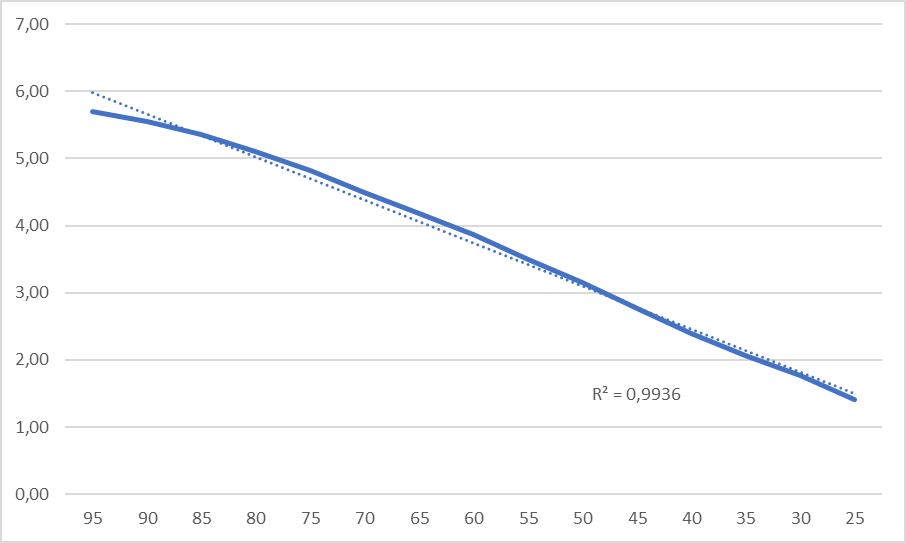
\includegraphics[scale=0.6]{src/imagenes/Grafica_NTC.png}
\label{fgr:Grafica_NTC}
\caption{Gráfica de la salida de tensión.}
\end{figure}

% Sensor de hilo caliente
\subsection{Medición de caudal con un sensor de hilo caliente}

El sensor de maza de flujo de aire convierte la cantidad de aire que entra al sistema en una señal de voltaje. El sistema tiene que saber el volumen de entrada de aire para calcular la cantidad de aire caliente necesario. El sensor de flujo de aire se encuentra directamente en la toma de aire de admisión. \\

Para poder medir los efectos de la variación de la resistividad con la temperatura, el circuito debe alimentarse con una corriente constante. Asi toda variacion de flujo o caudal se vera reflejada en una caida de tensión. El circuito para generar una corriente constante es el siguiente:

\begin{figure}[H]
\centering
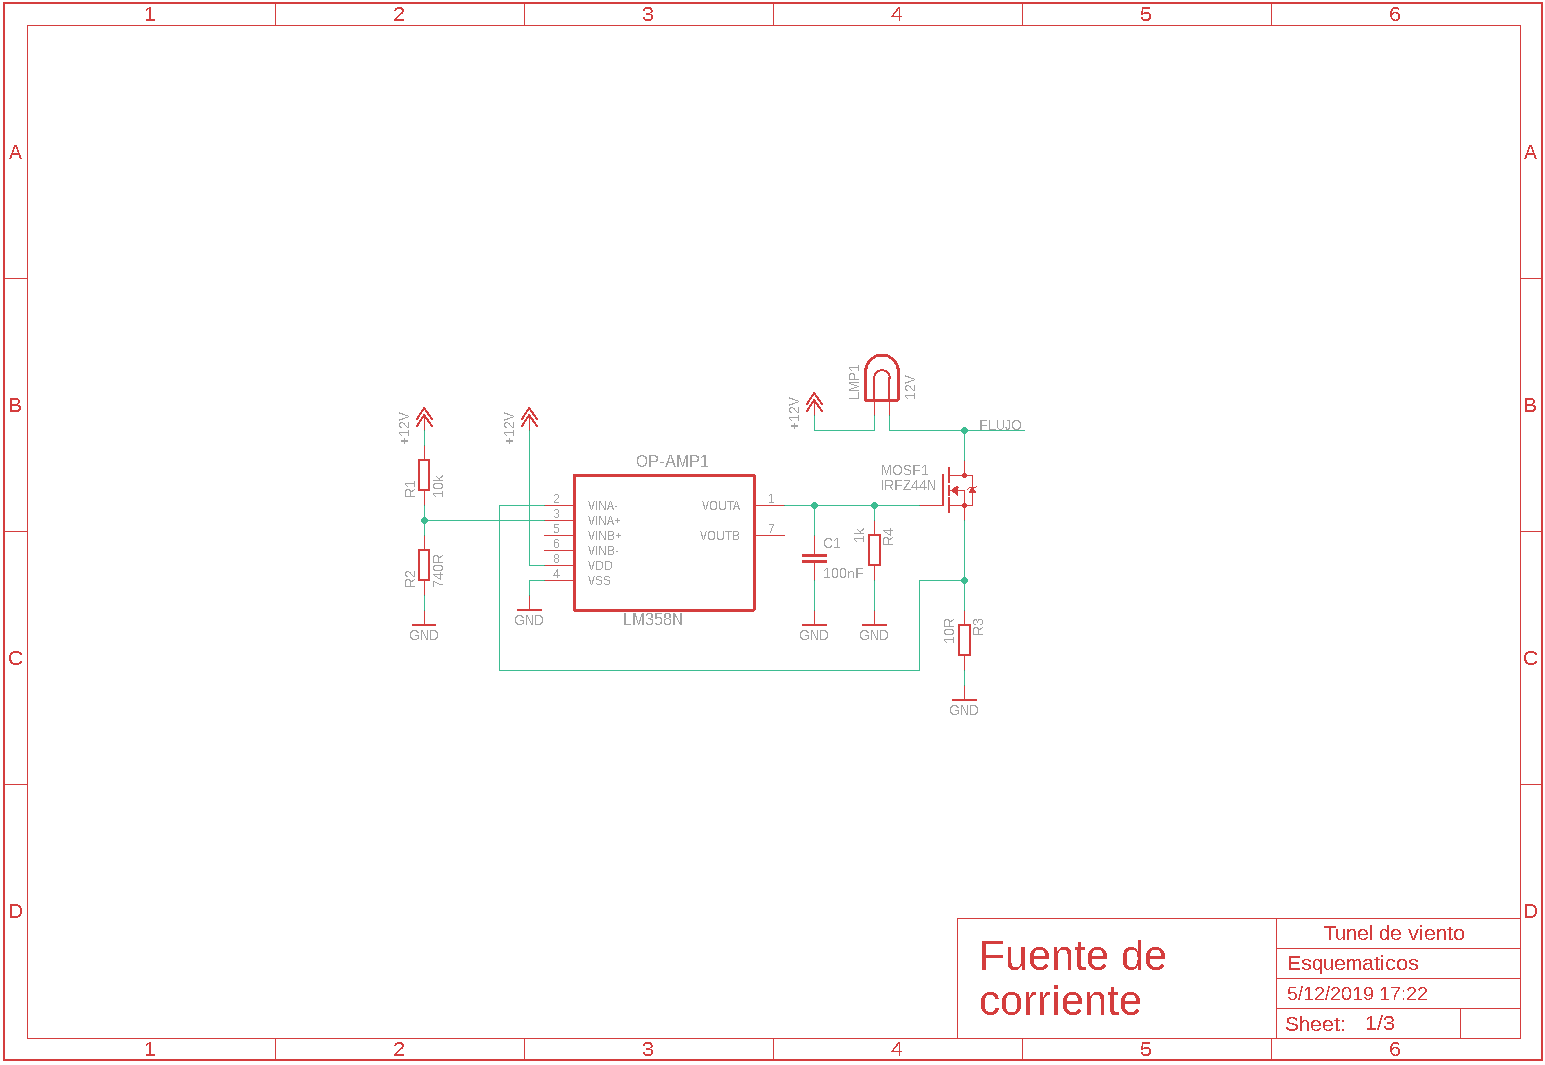
\includegraphics[scale=0.6]{src/imagenes/Fuente_de_corriente.png}
\label{fgr:Fuente_de_corriente}
\caption{Sensor de hilo caliente.}
\end{figure}

\begin{figure}[H]
\centering
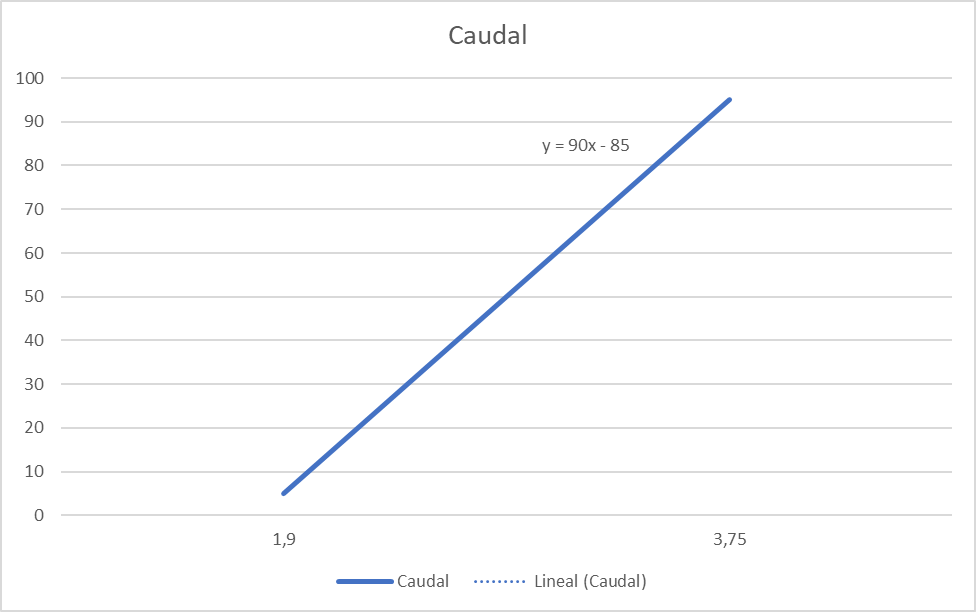
\includegraphics[scale=0.6]{src/imagenes/Grafica_hilo_caliente.png}
\label{fgr:Grafica_hilo_caliente}
\caption{Salida de voltaje del hilo caliente.}
\end{figure}

Expresando el caudal como un porcentaje entre el mínimo obtenido (sin los ventiladores encendidos) y el máximo (clapeta totalmente abierta con ventiladores al máximo), la siguiente gráfica muestra la salida de tensión en función al porcentaje. \\

Suponiendo un comportamiento lineal, la aproximación se utilizará para calcular la mezcla de aire frío con el caliente.

% Centro de control
\subsection{Centro de control}

\begin{figure}[H]
\centering
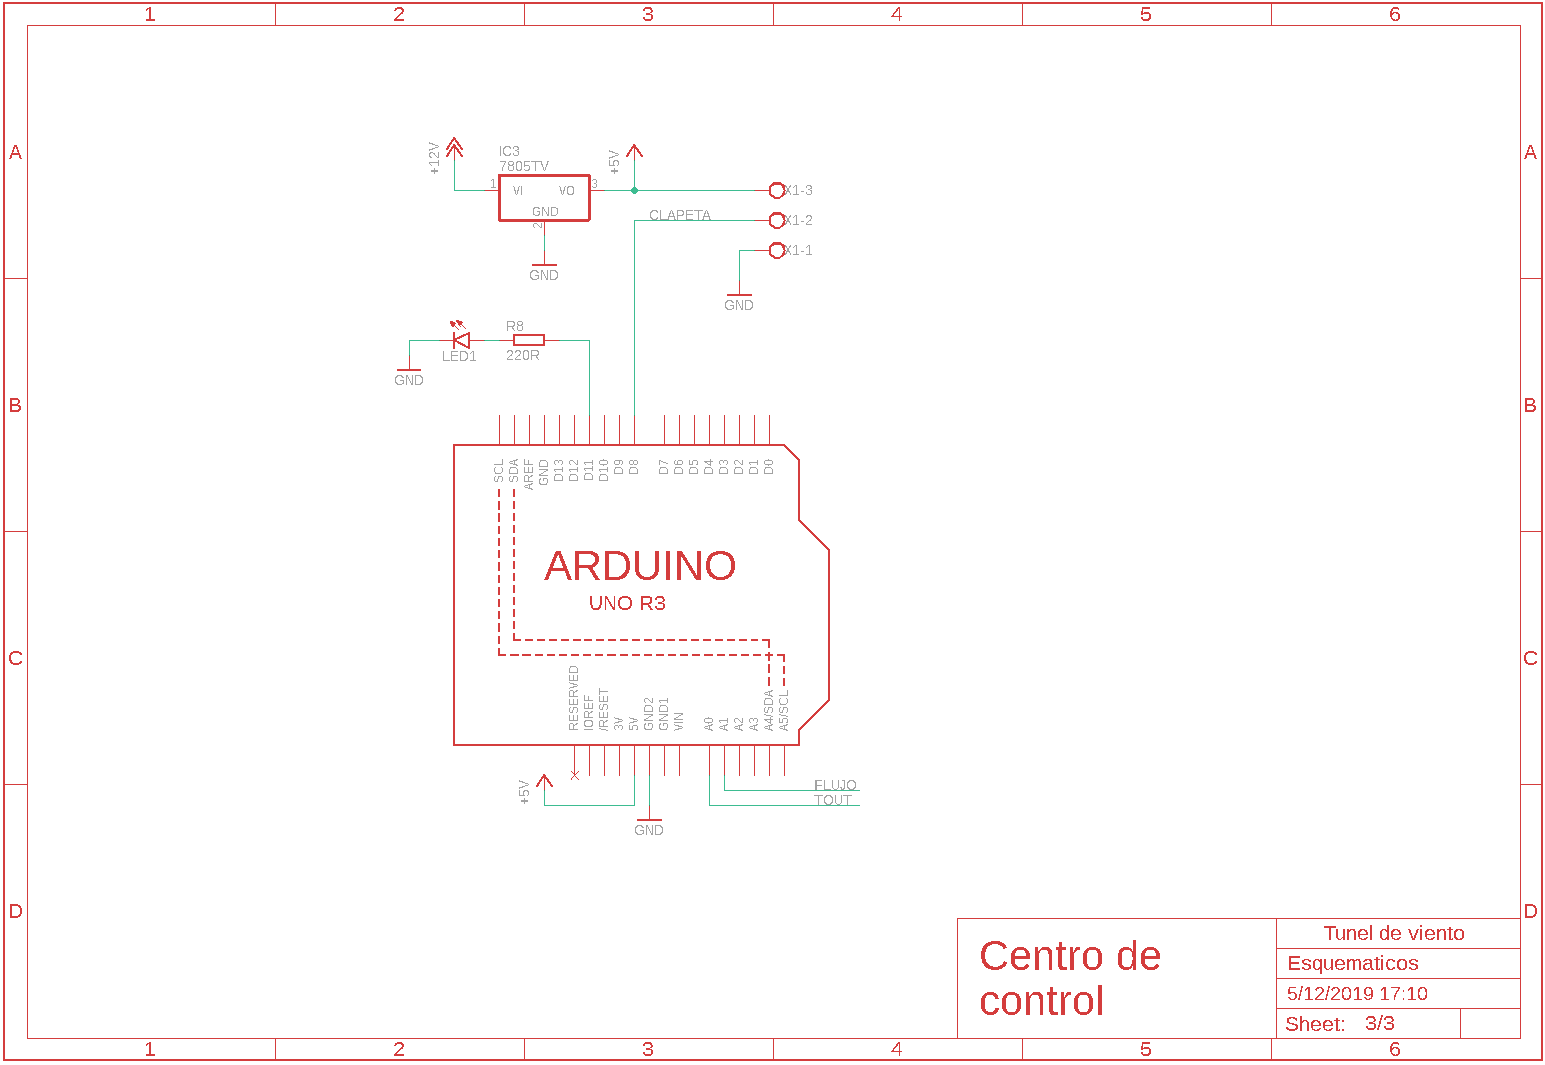
\includegraphics[scale=0.6]{src/imagenes/Centro_de_control.png}
\label{fgr:Centro_de_control}
\caption{Control del sistema con un Arduino UNO.}
\end{figure}

El centro de control de sistema es un Arduino UNO, que controla la posición de la clapeta de entrada de aire frío, que son realimentadas con dos entradas analógicas, la de temperatura y la de caudal. Posee un led de estado que cambia la frecuencia de parpadeo dependiendo el estado del sistema y envia comandos al HMI cada 1s para poder visualizar los parametros de salida y entrada.

% Protocolo de comunicacion
\subsubsection{Protocolo de comunicación Arduino HMI}
Para lograr la comunicacion del Arduino con el HMI, se utilizo el siguiente protocolo de comunicación con el formato correspondiente:

\begin{table}[H]
\begin{center}
\begin{tabular}{|l|l|l|}
\hline
\multicolumn{3}{|c|}{Cabecera} \\
\hline
Dato & Descripción & Tipo de dato \\
\hline
0x50 & 'P' & uint8\_t \\
\hline
0x44 & 'D' & uint8\_t \\
\hline
0x43 & 'C' & uint8\_t \\
\hline
0x43 & 'C' & uint8\_t \\
\hline
0xXX & Tamaño del payload & uint8\_t \\
\hline
0x3A & ':' Token & uint8\_t \\
\hline
\multicolumn{3}{|c|}{Ejecución de comandos} \\
\hline
0xXX & CMD comando a enviar & uint8\_t \\
\hline
0xXX & Array de payload & uint8\_t[x] \\
\hline
0xXX & Checksum & uint8\_t \\
\hline
\end{tabular}
\end{center}
\end{table}

Conocido este formato, el payload se enviara con el estandar Little Endian, es decir, primero se
transmite el byte menos significativo del número.

\begin{table}[H]
\begin{center}
\begin{tabular}{|l|l|l|l|}
\hline
ID & Dirección & Payload & Descripción \\
\hline
\multicolumn{4}{|c|}{Comandos de datos y control} \\
\hline
\multirow{2}{0pt}{0x00} & $PC \longrightarrow ARDUINO$ &  & Posición actual del servo \\
\cline{2-4} & $ARDUINO \longrightarrow PC$ & uint16\_t & Posición actual del servo en us \\
\hline
\multirow{2}{0pt}{0x01} & $PC \longrightarrow ARDUINO$ & int16\_t & Setear temperatura de salida \\
\cline{2-4} & $ARDUINO \longrightarrow PC$ & int16\_t & Temperatura de salida seteada \\
\hline
\multirow{2}{0pt}{0x02} & $PC \longrightarrow ARDUINO$ &  & Temperatura de salida \\
\cline{2-4} & $ARDUINO \longrightarrow PC$ & int16\_t & Temperatura de salida x 10 \\
\hline
\multirow{2}{0pt}{0x03} & $PC \longrightarrow ARDUINO$ &  & Caudal de salida \\
\cline{2-4} & $ARDUINO \longrightarrow PC$ & int16\_t & Caudal de salida x 10 \\
\hline
\multicolumn{4}{|c|}{Comandos de activación o especiales} \\
\hline
\multirow{2}{0pt}{0xFE} & $PC \longrightarrow ARDUINO$ &  & Ping \\
\cline{2-4} & $ARDUINO \longrightarrow PC$ &  & Ping \\
\hline
0xXX & $PC \longrightarrow ARDUINO$ &  & Comando invalido o error de checksum \\
\hline
0xFF & $ARDUINO \longrightarrow PC$ & uint8\_t & Comando invalido o error de checksum \\
\hline
\end{tabular}
\end{center}
\end{table}

% Imagenes del proyecto terminado
\section{Construcción}

% Circuitos de control y sensores
\subsection{Circuitos de control y sensores}

Se incorporo un led de estado para poder visualizar los estados del Arduino, al no tener pantalla el debug se complica mucho. Ademas sirve como advertencia al usuario ante un error no previsto.

\begin{figure}[H]
\centering
\includegraphics[scale=0.1, angle=-90]{src/imagenes/Control_Central.jpg}
\label{fgr:Control_Central}
\caption{Arduino.}
\end{figure}

Para poder controlar el servo se debe emitir un pulso que varia entre $1ms$ y $2ms$ con una frecuencia de $50Hz$, esto se pudo lograr no programando al microcontrolador con el IDE de Arduino, sino que programando en lenguaje C++ nativo. Los resultados logrados fueron muy buenos.

\begin{figure}[H]
\centering
\includegraphics[scale=0.08]{src/imagenes/Control_servo.jpg}
\label{fgr:Control_servo}
\caption{Control del servo.}
\end{figure}

\subsection{Fuente de corriente constante}

Para la construcción de la fuente de corriente se realizo el montaje en una protoboard y se probo la salida, variando un potenciometro para conseguir el ajuste manual de la corriente de alimentación en torno a los $60mA$.

\begin{figure}[H]
\centering
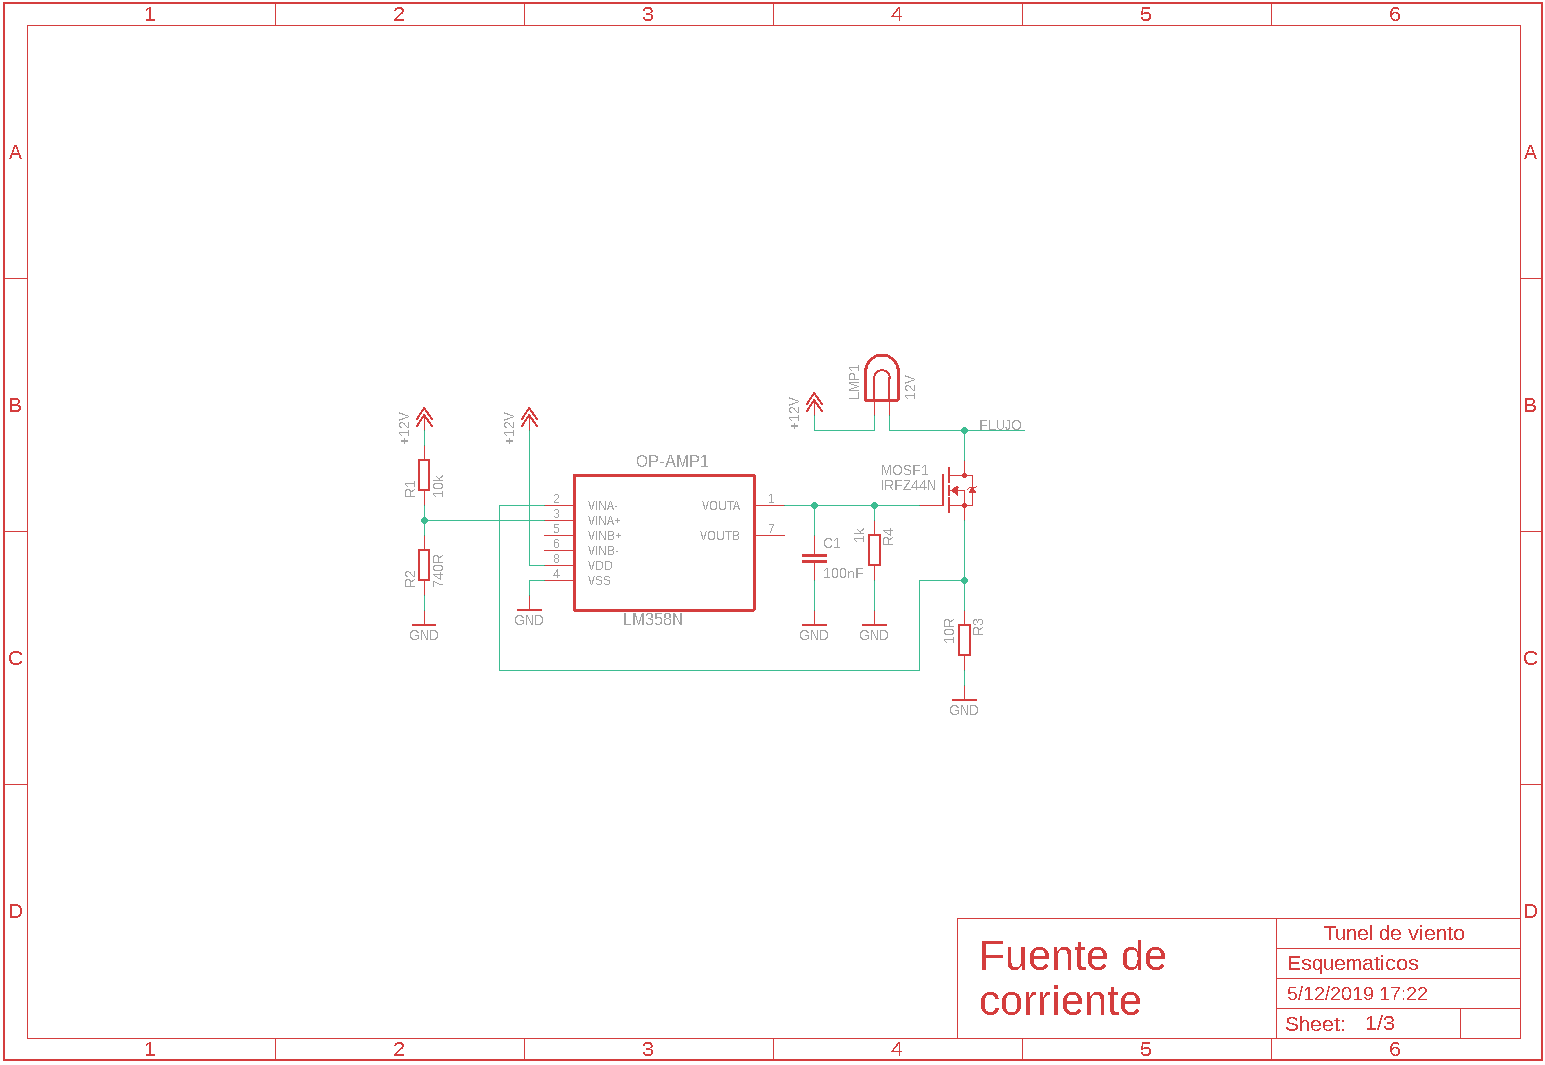
\includegraphics[scale=0.1, angle=-90]{src/imagenes/Fuente_de_corriente.jpg}
\label{fgr:Fuente_de_corriente}
\caption{Fuente de corriente.}
\end{figure}

% HMI
\subsection{HMI}

El Interfaz Hombre-Máquina (HMI) es el interfaz entre el proceso y los operario. Se trata básicamente de un panel de instrumentos del operario. Es la principal herramienta utilizada por operarios y supervisores de línea para coordinar y controlar procesos industriales y de fabricación. El HMI traduce variables de procesos complejos en información útil y procesable. \\

Como este sistema tiene que ser facilmente controlado y monitorizado, la interfaz que se desarrollo cumple con los requerimientos de operación.

\begin{figure}[H]
\centering
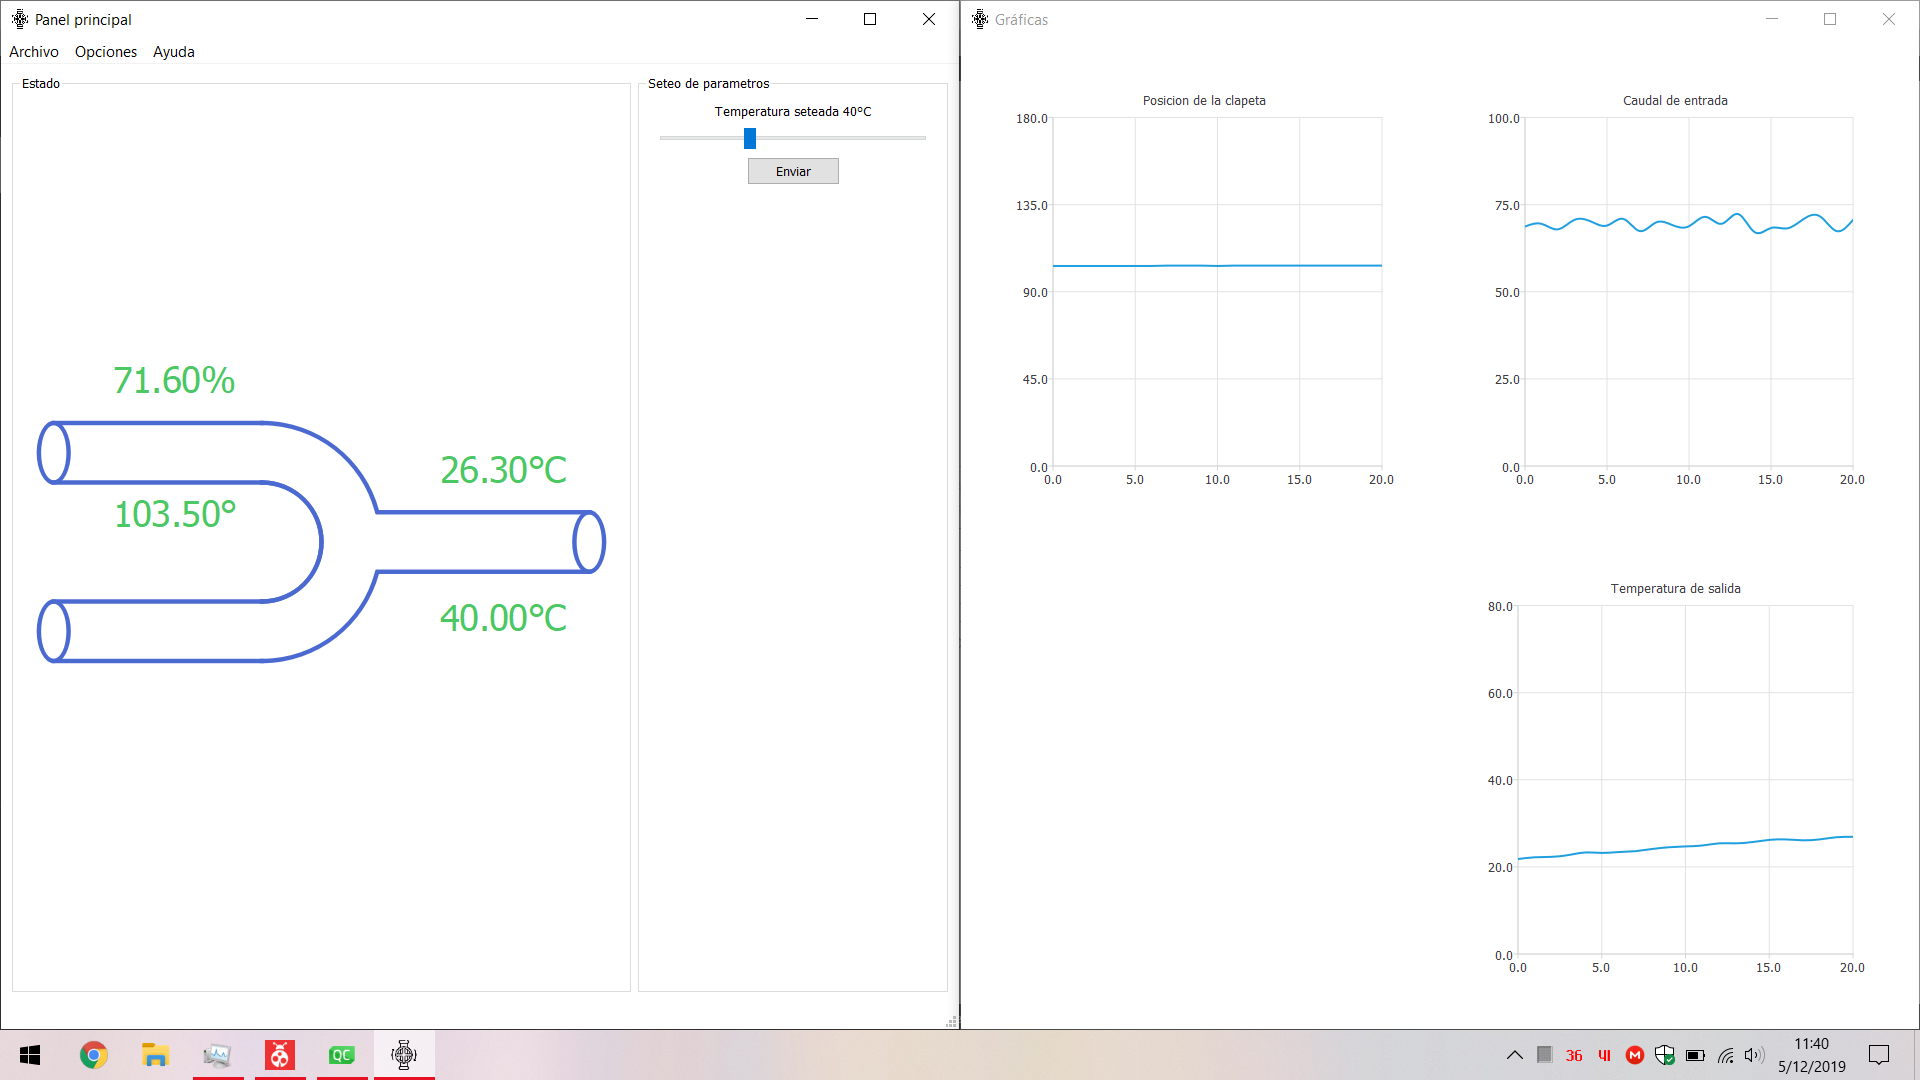
\includegraphics[scale=0.25]{src/imagenes/HMI_1.png}
\label{fgr:HMI_1}
\caption{HMI.}
\end{figure}

La función de los HMI consiste en mostrar información operativa en tiempo real y casi en tiempo real. Proporcionan gráficos de procesos visuales que aportan significado y contexto al estado del motor y de la válvula, niveles de depósitos y otros parámetros del proceso. Suministran información operativa al proceso, y permiten el controlar y la optimización al regular los objetivos de producción y de proceso. \\

A la izquierda se puede aprecial el sistema de forma gráfica, lo que permite saber que esta pasando en cada punto de operación. Mientras que a la derecha se muestran las gráficas y curvas de tendencia hasta 20 segundos antes.

\begin{figure}[H]
\centering
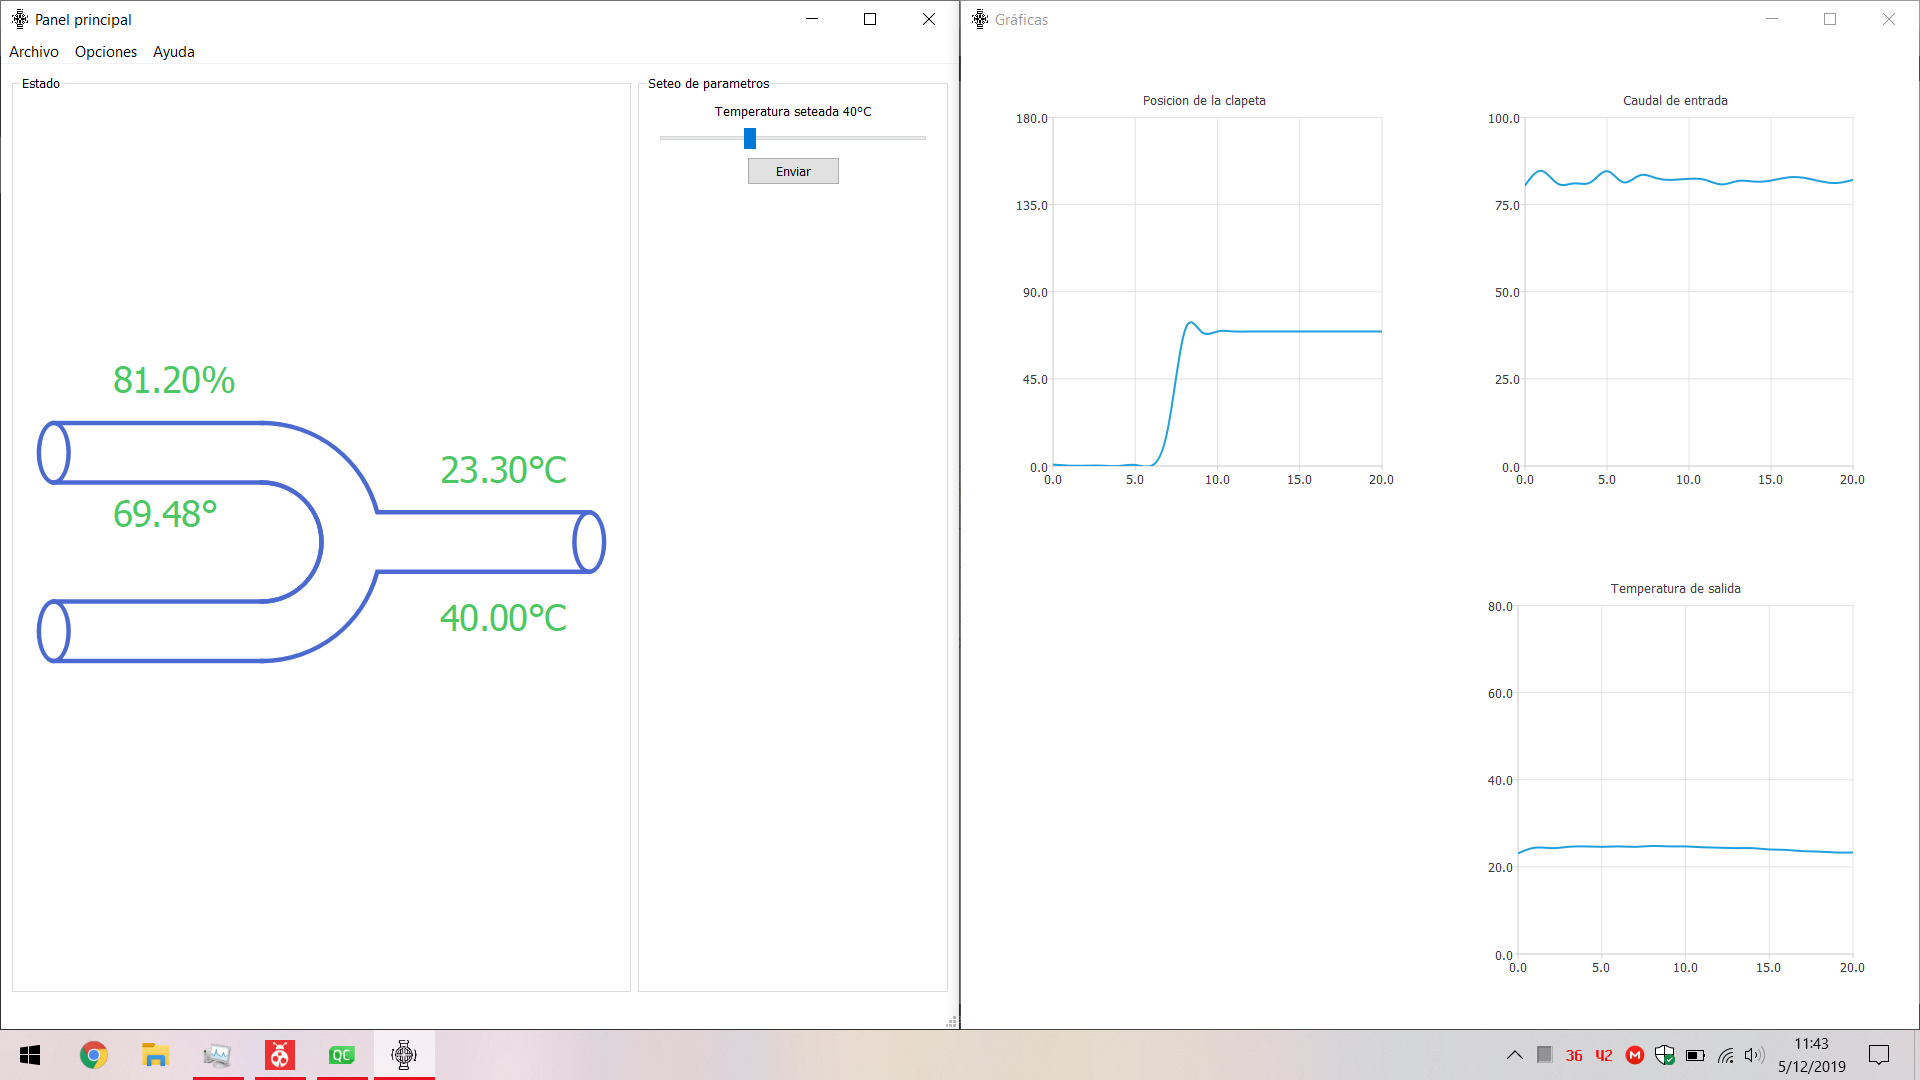
\includegraphics[scale=0.25]{src/imagenes/HMI_2.png}
\label{fgr:HMI_2}
\caption{HMI.}
\end{figure}

% Pruebas y resultados obtenidos
\section{Pruebas y resultados obtenidos}

\begin{figure}[H]
\centering
\includegraphics[scale=0.08, angle=-90]{src/imagenes/Sesor_patron.jpg}
\label{fgr:Sesor_patron}
\caption{Patron de temperatura.}
\end{figure}

\begin{figure}[H]
\centering
\includegraphics[scale=0.08, angle=-90]{src/imagenes/Sistema_prueba_1.jpg}
\label{fgr:Sitema_prueba_1}
\caption{Sitema armado casi completamente.}
\end{figure}

\begin{figure}[H]
\centering
\includegraphics[scale=0.08]{src/imagenes/Sistema_prueba_2.jpg}
\label{fgr:Sitema_prueba_2}
\caption{Prueba de software y curvas de respuesta.}
\end{figure}

% Conclusión y recomendaciones
\section{Conclusión y recomendaciones}

A lo largo del desarrollo del proyecto nos hemos topado con varios inconvenientes:

\begin{enumerate}
	\item Materiales de construcción.
	\item Adaptación de los sensores.
	\item Ruido eléctrico en todas las mediciones.
	\item Inercia termina (muy baja velocidad de respuesta).
\end{enumerate}

\end{document}